\renewcommand{\theequation}{\theenumi}
\renewcommand{\thefigure}{\theenumi}
\renewcommand{\thetable}{\theenumi}
\begin{enumerate}[label=\thesection.\arabic*.,ref=\thesection.\theenumi]
\numberwithin{equation}{enumi}
\numberwithin{figure}{enumi}
\numberwithin{table}{enumi}
%
\item Let $X$ be a non-negative integer valued random variable with probability mass function $f(x)$ satisfying $(x+1)f(x+1)=(\alpha + \beta x)f(x)$, $x=0,1,2,...$; $\beta \neq 1$. You may assume that $E(X)$ and $Var(X)$ exist. Then which of the following statements are true?

\begin{enumerate}
    \item $E(X)=\dfrac{\alpha}{1-\beta}$ \vspace{0.2cm}
    \item $E(X)=\dfrac{\alpha^2}{(1-\beta)(1+\alpha)}$ \vspace{0.2cm}
    \item $Var(X)=\dfrac{\alpha^2}{(1-\beta)^2}$ \vspace{0.2cm}
    \item $Var(X)=\dfrac{\alpha}{(1-\beta)^2}$
\end{enumerate}
%
\solution
For a discrete random variable $X$ with P.D.F. $f(x)$ and which can take values from a set $\mathbb{S}$,
\begin{align} \label{june2013-75:eq-1}
    E(X)= \sum_{x \in \mathbb{S}}xf(x)
\end{align}
And,
\begin{align} \label{june2013-75:eq-2}
    E(X^2) =\sum_{x \in \mathbb{S}}x^2f(x)
\end{align}
Also, as $f(x)$ is the P.D.F.,
\begin{align} \label{june2013-75:eq-3}
    \sum_{x \in \mathbb{S}}f(x) = 1
\end{align}
Given, for $x \in \mathbb{S}=\{0,1,2,...n\}$,
\begin{align} \label{june2013-75:eq-4}
    (x+1)f(x+1)=(\alpha + \beta x)f(x)
\end{align}
Summing both sides for $x \in \mathbb{S}$ we get,
\begin{align}
    \sum_{x=0}^n(x+1)f(x+1)=\sum_{x=0}^n(\alpha +\beta x)f(x)
\end{align}
Replacing $x+1$ with $x$ in L.H.S. we get, 
\begin{align}
    \sum_{x=1}^{n+1}xf(x)=\sum_{x=0}^n(\alpha +\beta x)f(x)
\end{align}
Rewriting LHS, we get,
\begin{align}
    \sum_{x=0}^nxf(x)+(n+1)f(n+1)=\sum_{x=0}^n(\alpha +\beta x)f(x)
\end{align}
But as $x \in \{0,1,2...n\}$, $f(n+1)=0$. So the equation becomes
\begin{align}
    \sum_{x=0}^nxf(x)=\alpha \sum_{x=0}^nf(x) + \beta \sum_{x=0}^nxf(x)
\end{align}
Using \eqref{june2013-75:eq-1} and \eqref{june2013-75:eq-3}, we get,
\begin{align} 
    E(X)=\alpha(1) + \beta E(X)
\end{align}
So,
\begin{align} \label{june2013-75:eq-5}
    E(X)=\dfrac{\alpha}{1-\beta}
\end{align}
Now in \eqref{june2013-75:eq-4}, multiplying both sides by $(x+1)$, we get,
\begin{align}
    (x+1)^2f(x+1)=(\alpha + \beta x)(x+1)f(x)
\end{align}
Summing both sides for $x \in \mathbb{S}$ we get,
\begin{align}
    \sum_{x=0}^n(x+1)^2f(x+1)=\sum_{x=0}^n(\alpha +\beta x)(x+1)f(x)
\end{align}
Replacing $x+1$ with $x$ in L.H.S. we get, 
\begin{align}
    \sum_{x=1}^{n+1}x^2f(x)=\sum_{x=0}^n(\beta x^2f(x) + (\alpha+\beta)xf(x) + \alpha f(x))
\end{align}
Rewriting LHS similarly as before, we get,
\begin{align}
    \sum_{x=0}^nx^2f(x)=\beta \sum_{x=0}^nx^2f(x) + \nonumber \\
    (\alpha + \beta)\sum_{x=0}^nxf(x) + \alpha \sum_{x=0}^nf(x)
\end{align}
Using \eqref{june2013-75:eq-1}, \eqref{june2013-75:eq-2} and \eqref{june2013-75:eq-3}, we get,
\begin{align}
    E(X^2)=\beta E(X^2) + (\alpha + \beta)E(X) + \alpha (1) 
\end{align}
Using \eqref{june2013-75:eq-5}
\begin{align}
    E(X^2)(1-\beta)=\dfrac{\alpha(\alpha+\beta)}{1-\beta} + \alpha
\end{align}
So,
\begin{align} \label{june2013-75:eq-6}
    E(X^2)=\dfrac{\alpha^2+\alpha}{(1-\beta)^2}
\end{align}
Now,
\begin{align}
    Var(X)=E(X^2)-(E(X))^2
\end{align}
Using \eqref{june2013-75:eq-5} and \eqref{june2013-75:eq-6},
\begin{align}
    Var(X)=\dfrac{\alpha^2+\alpha}{(1-\beta)^2}-\dfrac{\alpha^2}{(1-\beta)^2}
\end{align}
So,
\begin{align}
    Var(X)=\dfrac{\alpha}{(1-\beta)^2}
\end{align}
So, options 1 and 4 are correct.
%
\item Let X be a random variable with probability density function,
\begin{align}
    f(x)=\alpha(x-\mu)^{\alpha-1}e^{-(x-\mu)^{\alpha}}
\end{align}
such that $-\infty<\mu<\infty\;;\alpha>0\;;x>\mu$, The hazard function is: 
\begin{enumerate}
    \item constant for all $\alpha$
    \item an increasing function for some $\alpha$
    \item independent of $\alpha$
    \item independent of $\mu$ when $\alpha=1$
\end{enumerate}
%
\solution
Given PDF of X,
\begin{align}
    f(x)=\alpha(x-\mu)^{\alpha-1}e^{-(x-\mu)^{\alpha}}\label{june2014-71:3}
\end{align}
\textbf{Important property}(using in \eqref{june2014-71:1} as $x>\mu$):
Given $x-y>0$ and $-\infty<y<\infty$, then
\begin{align}
    \lim_{x \to -\infty} x-y=0
\end{align}
CDF of X,
\begin{align}
    F(x)&=\int_{-\infty}^x{f(x)\;dx}\\
    &=\int_{-\infty}^x{\alpha(x-\mu)^{\alpha-1}e^{-(x-\mu)^{\alpha}}dx}\\
    &=\int_{-\infty}^x{e^{-(x-\mu)^{\alpha}}d(x-\mu)^{\alpha}}\\
    &=\sbrak{\frac{e^{-(x-\mu)^{\alpha}}}{-1}}_{-\infty}^x\\
    &=-e^{-(x-\mu)^{\alpha}}-\lim_{x \to -\infty} \frac{e^{-(x-\mu)^{\alpha}}}{-1}\label{june2014-71:1}\\
    &=-e^{-(x-\mu)^{\alpha}}+ {e^{-(0)^{\alpha}}}\\
   F(x) &=1-e^{-(x-\mu)^{\alpha}}\label{june2014-71:2}
\end{align}
Hazard function $\beta(x)$,(using \eqref{june2014-71:3} and \eqref{june2014-71:2})
\begin{align}
    \beta(x)&=\frac{f(x)}{1-F(x)}\\
    &=\frac{\alpha(x-\mu)^{\alpha-1}e^{-(x-\mu)^{\alpha}}}{1-(1-e^{-(x-\mu)^{\alpha}})}\\
    &=\frac{\alpha(x-\mu)^{\alpha-1}e^{-(x-\mu)^{\alpha}}}{e^{-(x-\mu)^{\alpha}}}\\
    \beta(x)&=\alpha(x-\mu)^{\alpha-1}
\end{align}
\begin{enumerate}
    \item $\beta(x)$ is not constant for all $\alpha$
    \item $\beta(x)=\alpha(x-\mu)^{\alpha-1}$ is an increasing function for $\alpha<0 \;or\; \alpha>1$ as given $x-\mu>0$ for all x.
    
    \textbf{Proof: }
    Using first derivative test, A function is increasing iff its first derivative is positive for all x. 
    \begin{align}
        \dfrac{d}{dx} \beta(x)&=  \dfrac{d}{dx} \alpha(x-\mu)^{\alpha-1}\\
        &= \alpha(\alpha-1)(x-\mu)^{\alpha-2}\label{june2014-71:0}
    \end{align}
    For \eqref{june2014-71:0} to be positive, (As given $x-\mu>0$)
    \begin{align}
        \alpha(\alpha-1)(x-\mu)^{\alpha-2}&>0\\
        \alpha(\alpha-1)&>0\\
        \implies \alpha \in \brak{-\infty,0}\cup \brak{1,\infty}
    \end{align}
    $\therefore \beta(x)$ an increasing function for some $\alpha$
    \item $\beta(x)$ is dependent of $\alpha$
    \item when $\alpha=1$,
\begin{align}
    \beta(x)&=\alpha(x-\mu)^{0}=\alpha
\end{align}
Therefore the hazard function is independent of $\mu$ when $\alpha=1$.
\end{enumerate}
\textbf{ANSWER: (2) and (4)}
%
\item 
A point is chosen at random from a circular disc shown below. What is the probability that the point lies in the sector OAB?\\

\begin{tikzpicture}
\draw (0,0) circle (3cm);
\draw (0,0) node{O}-- (2,2.25) node{A};
\draw (0,0) -- (2.828,1) node{B};
\end{tikzpicture}\\

( where $\angle$AOB = x radians )


    \begin{enumerate}
        \item $\frac{2x}{\pi}$
        \item $\frac{x}{\pi}$
        \item $\frac{x}{2\pi}$
        \item $\frac{x}{4\pi}$
    \end{enumerate}

%
\solution
\section*{\textbf{solution}}
Let $X \in \{0,1\}$ be a random variable such that X=0 means we choose a point lying in sector OAB and X=1 means that we choose a point lying outside sector OAB and inside the circle.\\

Area of a sector subtending an angle $\theta$ at the centre of circle with radius a is given by :
\begin{equation}
    A = \frac{1}{2}a^2\theta
\end{equation}
where $\theta$ is in radians.\\

Let the radius of circle shown in figure be r. It is given that  sector  OAB subtends an angle of x radians at the centre of the circle.\\

Probability that the chosen point lies in sector OAB is:
\begin{align}
    \pr{X=0} =& \frac{\text{Area of sector OAB}}{\text{Area of circle}}\\
       =& \frac{\frac{1}{2} r^2 x}{\pi r^2}\\
       =& \frac{x}{2\pi}
\end{align}

$\therefore$The correct answer is \textbf{option (3)} $\frac{x}{2\pi}$.

\section*{\textbf{alternate solution}}
The joint pdf is given by:
\begin{equation}
 \texorpdfstring{f\textsubscript{r$\theta$}}{f r $\theta$}(r,\theta)= \begin{cases}
                        \dfrac{r}{\pi R^2}  & \text{if 0 $<$ r $<$ R , 0 $<$ $\theta$ $<$ 2$\pi$ }\\
                        0  & \text{otherwise}
                        \end{cases}
\end{equation}

Let A $\equiv$ (R,  $\theta _2$) and B $\equiv$ (R,  $\theta _1$). \\
Hence,
\begin{equation}
(\theta _2 - \theta _1)= x    
\end{equation}

We want $\theta$ $\in$ ($\theta _1$ , $\theta _2$) and r $\in$ (0,R) for point to lie in the sector.
Let the point to be chosen be (r, $\theta$).\\

So, Required probability is:
\begin{align}
 \nonumber  \pr{\theta_1<\theta<\theta_2 , 0<r<R}\\
    =& \Int_{\theta_1}^{\theta_2} \Int_{0}^{R} \dfrac{r}{\pi R^2} \,dr\,d\theta \\
    =& \Int_{\theta_1}^{\theta_2} \dfrac{1}{\pi R^2} \dfrac{r^2}{2} \Bigg|_0^R \\
    =& \Int_{\theta_1}^{\theta_2} \dfrac{R^2}{2\pi R^2} \,d\theta  \displaybreak  \\
    =& \Int_{\theta_1}^{\theta_2} \dfrac{1}{2\pi} \,d\theta\\
    =& \dfrac{\theta}{2\pi} \Bigg|_{\theta_1}^{\theta_2} \\
    =& \dfrac{\theta_2 - \theta_1}{2\pi} \\
    =& \dfrac{x}{2\pi}
\end{align}
    
$\therefore$The correct answer is \textbf{option (3)} \Large $\frac{x}{2\pi}$.


%
\item Let $X$ and $Y$ be independent random variables each following a uniform distribution on $(0,1)$.Let $W=XI_{\{Y\leq X^2\}}$,where $I_A$ denotes the indicator function of set $A$.Then which of the following statements are true? \\
\begin{enumerate}
\item The cumulative distribution function of $W$ is given by
\begin{align}
  F_W(t)=t^2I_{\{0\leq t \leq 1\}}+ I_{\{t > 1\}}
\end{align}
\item $P\sbrak{W>0}=\frac{1}{3}$
\item The cumulative distribution function of $W$ is continuous
\item The cumulative distribution function of $W$ is given by
\begin{align}
  F_W(t)=\brak{\frac{2+t^3}{3}}I_{\{0\leq t \leq 1\}}+ I_{\{t > 1\}}
\end{align}
\end{enumerate}
%
\solution






Given $X$ and $Y$ are two independent random\\
variables. \\
Given $W=XI_{\{Y\leq X^2\}}$ \\
$X \in \brak{0,1}$ , $Y \in \brak{0,1}$ , $W \in [0,1)$\\
\begin{enumerate}
\item We need to find CDF of $W$
\begin{enumerate}
\item The PDF for $X$ is
\begin{align}
p_X(x) = 
\begin{cases}
     1 & 0 < x  < 1 \\
     0 & otherwise 
\end{cases}\label{june2013-70:1}
\end{align}
\item The CDF for $X$ is
\begin{align}
F_{X}(x)  = 
\begin{cases}
      0 & x \leq 0 \\
      x & 0 < x < 1 \\
      1 & otherwise
\end{cases}  \label{june2013-70:eq:2}
\end{align}
\item The PDF for $Y$ is
\begin{align}
p_{Y}(y)  = 
\begin{cases}
      1 & 0 < y < 1 \\
      0 & otherwise 
\end{cases} \label{june2013-70:3}
\end{align}
\item The CDF for $Y$ is
\begin{align}
F_{Y}(y)  = 
\begin{cases}
      0 & y \leq 0 \\
      y & 0 < y < 1 \\
      1 & otherwise 
\end{cases}\label{june2013-70:4}
\end{align}
\item $I_{\{Y\leq X^2\}}$ is defined as follows
\begin{align} 
I_{\{Y\leq X^2\}} =
\begin{cases}
    1 & y \leq x^2  \\
    0 & otherwise 
\end{cases} \label{june2013-70:5}
\end{align}
\item $W$ is defined as follows
\begin{align}
W  = 
\begin{cases}
    x & y \leq x^2 \\
    0 & otherwise
\end{cases}  \label{june2013-70:6}
\end{align}
From \eqref{june2013-70:6}
\begin{align}
p_W(W=0) &= \Pr(I_{\{Y\leq X^2\}}=0) \\
         &=\Pr(x^2 <y) \label{june2013-70:7}
\end{align}
\item Let $Z=X^2-Y$ be a random variable where $Z \in \brak{-1,1}$

\begin{align}
F_{X^2}(u)&=\Pr(X^2 \leq u) \\
          &=\Pr(X \leq \sqrt{u}) \\
          &=F_X(\sqrt{u}) \label{june2013-70:8}
\end{align}
\begin{enumerate}
\item From \eqref{june2013-70:eq:2},The CDF for $X^2$ is
\begin{align}
F_{X^2}(u)  = 
\begin{cases}
      0 & u \leq 0 \\
      \sqrt{u} & 0 < u < 1 \\
      1 & otherwise
\end{cases} \label{june2013-70:9}
\end{align}
\item The PDF for $X^2$ is
\begin{align}
p_{X^2}(u)  = 
\begin{cases}
      \frac{1}{2\sqrt{u}} & 0 < u < 1 \\
      0 & otherwise
\end{cases} \label{june2013-70:10}
\end{align}
\begin{align}
F_{\{-Y\}}(v)&=\Pr(-Y \leq v) \\
          &=\Pr(Y \geq -v) \\
          &=1-F_Y(-v) \label{june2013-70:11}
\end{align}
\item From \eqref{june2013-70:4},The CDF for $(-Y)$ is
\begin{align}
F_{\{-Y\}}(v)  = 
\begin{cases}
      0 & v \leq -1\\
      1+v & -1 < v < 0 \\
      1 & otherwise 
\end{cases}\label{june2013-70:12}
\end{align}
\item The PDF for $(-Y)$ is
\begin{align}
p_{\{-Y\}}(v)  = 
\begin{cases}
      1 & -1 < v < 0 \\
      0 & otherwise
\end{cases} \label{june2013-70:p-y}
\end{align}
\item $Z=X^2-Y$ $\implies  z=u+v$\\
Using convolution
\begin{align}
p_Z(z)=\int_{- \infty}^{\infty} p_{X^2}(z-v)p_{\{-Y\}}(v) \mathrm{dv} \label{june2013-70:pz}
\end{align}
Solving \eqref{june2013-70:pz} using \eqref{june2013-70:p-y},\eqref{june2013-70:10} for $z \in (-1,1)$, we get PDF of $Z$ as follows
\begin{align}
p_{Z}(z)  = 
\begin{cases}
      \sqrt{z+1} & -1 < z \leq 0 \\
      1-\sqrt{z} & 0 < z <1 \\
      0 & otherwise 
\end{cases} \label{june2013-70:13}
\end{align}
\item CDF of $Z$ as follows
\begin{align}
F_{Z}(z)  = 
\begin{cases}
      \frac{2}{3}{(z+1)}^\frac{3}{2} & -1 < z \leq 0 \\
      z-\frac{2}{3}{z}^\frac{3}{2} & 0 < z < 1 \\
      1 & otherwise
\end{cases} \label{june2013-70:14}
\end{align}

\end{enumerate}

\item using \eqref{june2013-70:14} to find $p_W(W=0)$
\begin{align}
p_W(W=0) &=\Pr(x^2 <y) \\
         &=F_z(0) \\
         &=\frac{2}{3} \label{june2013-70:15}
\end{align}

\item $W=t \implies X=t $ where $t \in (0,1)$
\begin{align}
p_{W}(t) = \int_{- \infty}^{\infty} p_X(t)I_{\{y\leq t^2\}} \mathrm{dy}
\end{align}
\begin{align}
   0 &< y < 1 \label{june2013-70:16} \\
   0 &< y \leq t^2  \label{june2013-70:17}
\end{align}
For $ 0 < t < 1 $,
\begin{align}
p_W(t) &= \int_{0}^{t^2} p_X(t)I_{\{y\leq t^2\}} \mathrm{dy} \\
       &= t^2 \label{june2013-70:18}
\end{align}
\item $\therefore$ PDF of $W$ is as follows
\begin{align}
p_{W}(t)  = 
\begin{cases}
  \frac{2}{3}& t=0 \\
  t^2 & 0 < t < 1 \\
  0 & otherwise
\end{cases} \label{june2013-70:19}
\end{align}
\item The CDF  of $W$ is as follows:
\begin{align}
F_W(t)  = 
\begin{cases}
  0 & t<0 \\
  \frac{2+t^3}{3}& 0 \leq t\leq 1\\
  1 & otherwise
\end{cases} \label{june2013-70:20}
\end{align}
\end{enumerate}
\item We need to find $P\sbrak{W>0}$
\begin{align}
\Pr(W > 0)&= 1- F_W(0) \\
           &=\frac{1}{3} \label{june2013-70:21} \\
\therefore \Pr(W>0)&=\frac{1}{3}
\end{align}
\item CDF of $W$ is discontinuous at $W=0$.\\
$\therefore$ option $3$ is incorrect.\\
\item The CDF in \eqref{june2013-70:20} can be written as
\begin{align}
  F_W(t)=\brak{\frac{2+t^3}{3}}I_{\{0\leq t \leq 1\}}+ I_{\{t > 1\}}
\end{align}
$\therefore$ option $2$ and $4$ are correct.
\begin{figure}[htb!]
\begin{center}
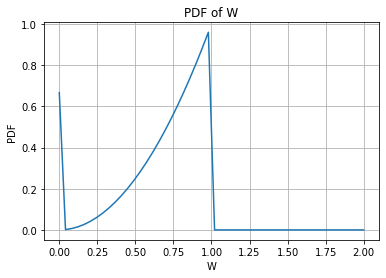
\includegraphics[width=\columnwidth]{solutions/2013/june/70/figures/assignment8pdf.png}
\end{center}
\end{figure}

\begin{figure}[htb!]
\begin{center}
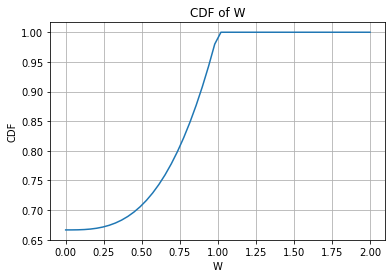
\includegraphics[width=\columnwidth]{solutions/2013/june/70/figures/assignment8cdf.png}
\end{center}
\end{figure}
\end{enumerate}

%
\item Let $U_1,U_2\dots,U_n$ be independent and identically distributed random variables each
having a uniform distribution on (0,1). Then,$\lim_{n \to +\infty} \pr{U_1+U_2\dots,U_n\leq \frac{3}{4}n}$
\begin{enumerate}
    \item does not exist
    \item exists and equals 0
    \item exists and equals 1
    \item exists and equals $\frac{3}{4}$
\end{enumerate}
%
\solution
We use Weak law for large numbers to solve this problem. 
Let the collection of identically distributed random variables $U_1,U_2\dots,U_n$
have a finite mean $\mu$ and finite variance $\sigma^2$.
\begin{align}
    \mu = \mean{U_i} \hspace{0.3cm}\text{for i $\in$ (1,2,3\dots,n)}\label{june2013-59:0.0.1}
\end{align}
Since the distribution is uniform on (0,1), $\mu$ = 0.5. Let $M_n$ be the sample mean
\begin{align}
     M_n = \frac{U_1+U_2+U_3\dots+U_n}{n}\label{june2013-59:0.0.2}
\end{align}
Expected value of $M_n$ (using \eqref{june2013-59:0.0.2} and \eqref{june2013-59:0.0.1})is
\begin{align}
    \mean{M_n} = &\frac{\mean{U_1+U_2+U_3+\dots+U_n}}{\mean{n}}\\[0.3cm]
     = &\frac{\mean{U_1}+\mean{U_2}+\dots+\mean{U_n}}{n}\\
     = &\frac{n\times\mu}{n}\\
     = & \mu
\end{align}
Variance of M
\begin{align}
    Var(M_n) =& \frac{Var(U_1+U_2+U_3\dots+U_n)}{n^2}\\[0.3cm]
    =& \frac{Var(U_1) + Var(U_2)\dots+Var(U_n)}{n^2}\\
    =& \frac{n\times{\sigma^2}}{n^2}\\[0.3cm]
    =& \frac{\sigma^2}{n} \label{june2013-59:0.0.10}
\end{align}
From Chebyshev inequality, for any $\epsilon > 0$
\begin{align}
    \pr{\abs{M_n-\mu}\geq \epsilon} \hspace{0.2cm} \leq \hspace{0.2cm} \frac{Var(M_n)}{\epsilon^2}
\end{align}
From \eqref{june2013-59:0.0.1} and \eqref{june2013-59:0.0.10}
\begin{align}
    \pr{\abs{\frac{U_1+U_2\dots+U_n}{n} - \mu} \geq \epsilon} \leq \frac{\sigma^2}{n\times\epsilon^2}\notag
\end{align}
\begin{align}
    \begin{split}
    \lim_{n \to \infty} \pr{\abs{\frac{U_1+U_2\dots+U_n}{n} - \mu} \geq \epsilon}\\
    \leq \lim_{n \to \infty} \frac{\sigma^2}{n\times\epsilon^2} \leq 0 \hspace{0.2cm} \text{for fixed $\epsilon > 0$}
    \end{split}
\end{align}
But since Probabilities are always non-negative,
\begin{align}
    \lim_{n \to \infty} \pr{\abs{\frac{U_1+U_2\dots+U_n}{n} - \mu} \geq \epsilon} \to 0 \label{june2013-59:0.0.13}
\end{align}
This is known as the weak law of large numbers\\
The inverse of \eqref{june2013-59:0.0.13} is also true
\begin{align}
    &\lim_{n \to \infty} \pr{\abs{\frac{U_1+U_2\dots+U_n}{n} - \mu} \leq \epsilon} \to 1 \\[0.3cm]
    &\abs{\frac{U_1+U_2\dots+U_n}{n} - \mu} \leq \epsilon \hspace{0.2cm}\text{as  n $\to$ $\infty$} 
\end{align}
From $\epsilon$, n definition of limits, it is clear that 
\begin{align}
    &\frac{U_1+U_2\dots+U_n}{n} \to \mu\\
    &U_1+U_2\dots U_n \to n\times\mu \hspace{0.2cm}\text{as  n $\to$ $\infty$}
\end{align}
Since $\mu = \frac{1}{2}$,
\begin{align}
    \lim_{n \to +\infty} U_1+U_2\dots U_n = \frac{1}{2}n < \frac{3}{4}n
\end{align}
So 
\begin{align}
    \lim_{n \to +\infty} \pr{U_1+U_2\dots,U_n\leq \frac{3}{4}n} = 1
\end{align}
%
\item  Consider the quadratic equation $x^2+2U x+V=0$ where $U$ and $V$ are chosen independently and randomly from $\{1,2,3\}$ with equal probabilities. Then probability that the equation has both roots real
\begin{enumerate}
    \item $\frac{2}{3}$
    \item $\frac{1}{2}$
    \item $\frac{7}{9}$
    \item $\frac{1}{3}$
\end{enumerate}
%
\solution
Let $U\in\{1.2,3\}$ and $V\in\{1,2,3\}$
\begin{table}[h!]
\centering
\caption{Probability of selecting values for $U$}
\resizebox{\columnwidth}{!}{
  \begin{tabular}{||c|c|c|c||}
    \hline
    $k$ & $1$ & $2$ & $3$\\
    \hline
    \hline
    $\pr{U=k}$ & $1/3$ & $1/3$ & $1/3$\\
    \hline
  \end{tabular}
}
\label{june2013-60:Table1}
\end{table}
\begin{table}[h!]
\centering
\caption{Probability of selecting values for $V$}
\resizebox{\columnwidth}{!}{
  \begin{tabular}{||c|c|c|c||}
    \hline
    $k$ & $1$ & $2$ & $3$\\
    \hline
    \hline
    $\pr{V=k}$ & $1/3$ & $1/3$ & $1/3$\\
    \hline
  \end{tabular}
}
\label{june2013-60:Table2}
\end{table}
For $x^2+2U x+V=0$ to have real roots,
\begin{align}
    b^2-4ac\geq0\\
    \brak{2U}^2-4\brak{1}\brak{V}\geq0\\
    U^2\geq V
\end{align}
\begin{align}
    \pr{U^2\geq V}=1-\pr{U^2<V}
\end{align}
The possible pairs \brak{U,V} for \pr{U^2<V},
\vspace{0.00001in}
\begin{table}[h!]
\centering
\caption{Table for \pr{U^2<V}}
\resizebox{\columnwidth}{!}{
  \begin{tabular}{||c|c||}
    \hline
    $\brak{U,V}$ for $U^2<V$ & Probability\\
    \hline
    \hline
    $\brak{1,2}$ & \pr{U=1}\pr{V=2}=1/9\\
    \hline
    $\brak{1,3}$ & $\pr{U=1}\pr{V=3}=\frac{1}{9}$\\
    \hline
    \hline
    Total & $\pr{U^2<V}=\frac{2}{9}$\\
    \hline
  \end{tabular}
}
\label{june2013-60:Table3}
\end{table}
\begin{align}
    \pr{U^2\geq V}=1-\frac{2}{9}\\
    \pr{U^2\geq V}=\frac{7}{9}
\end{align}
Hence, Option 3 is correct.

%
\newcommand{\tikzAngleOfLine}{\tikz@AngleOfLine}
  \def\tikz@AngleOfLine(#1)(#2)#3{%
  \pgfmathanglebetweenpoints{%
    \pgfpointanchor{#1}{center}}{%
    \pgfpointanchor{#2}{center}}
  \pgfmathsetmacro{#3}{\pgfmathresult}%
  }

\item A point is chosen at random from a circular disc shown below. What is the probability that the point lies in the sector OAB?\\
\begin{tikzpicture}[
    colorstyle/.style={
       circle, draw=black,fill=black,
       thick, inner sep=0pt, minimum size=2 mm,
       outer sep=0pt
        },
    scale=2]
\draw (0,0) circle (2cm);
\node at (0,0) [colorstyle,label=below:O]{};
\node at (1,1.732) [colorstyle,label=above:A]{};
\node at (1.732,1) [colorstyle,label=above right:B]{};
\draw (0,0) -- (1,1.732);
\draw (0,0) -- (1.732,1);
\coordinate (O) at (0,0);
\coordinate (A) at (1,1.732);
\coordinate (B) at (1.732,1);
\tikzAngleOfLine(O)(B){\AngleStart}
    \tikzAngleOfLine(O)(A){\AngleEnd}
    \draw[red,<->] (O)+(\AngleStart:1cm) arc (\AngleStart:\AngleEnd:1 cm);
    \node[circle,fill=green] at ($(O)+({(\AngleStart+\AngleEnd)/2}:1.5 cm)$) {x};
\end{tikzpicture}\\
( where $\angle$AOB = x radians )
\begin{multicols}{2}
    \begin{enumerate}
        \item $\frac{2x}{\pi}$
        \item $\frac{x}{\pi}$
        \item $\frac{x}{2\pi}$
        \item $\frac{x}{4\pi}$
    \end{enumerate}
\end{multicols}
%
\solution
The joint pdf is given by:
\begin{equation}
 \texorpdfstring{f\textsubscript{r$\theta$}}{f r $\theta$}(r,\theta)= \begin{cases}
                        \dfrac{r}{\pi R^2}  & \text{if 0 $<$ r $<$ R , 0 $<$ $\theta$ $<$ 2$\pi$ }\\
                        0  & \text{otherwise}
                        \end{cases}
\end{equation}
Let A $\equiv$ (R,  $\theta _2$) and B $\equiv$ (R,  $\theta _1$). \\
Hence,
\begin{equation}
(\theta _2 - \theta _1)= x    
\end{equation}
We want $\theta$ $\in$ ($\theta _1$ , $\theta _2$) and r $\in$ (0,R) for point to lie in the sector.
Let the point to be chosen be (r, $\theta$).\\
So, Required probability is:
\begin{align}
 \nonumber  \pr{\theta_1<\theta<\theta_2 , 0<r<R}\\
    =& \Int_{\theta_1}^{\theta_2} \Int_{0}^{R} \dfrac{r}{\pi R^2} \,dr\,d\theta \displaybreak \\
    =& \Int_{\theta_1}^{\theta_2} \dfrac{1}{\pi R^2} \dfrac{r^2}{2} \Bigg|_0^R \\
    =& \Int_{\theta_1}^{\theta_2} \dfrac{R^2}{2\pi R^2} \,d\theta   \\
    =& \Int_{\theta_1}^{\theta_2} \dfrac{1}{2\pi} \,d\theta\\
    =& \dfrac{\theta}{2\pi} \Bigg|_{\theta_1}^{\theta_2} \\
    =& \dfrac{\theta_2 - \theta_1}{2\pi} \\
    =& \dfrac{x}{2\pi}
\end{align}
    
$\therefore$The correct answer is \textbf{option (3)} \Large $\frac{x}{2\pi}$.

%
\item Consider a parallel system with two components. The lifetimes of the two components are independent and identically distributed random variables each following an exponential distribution with mean 1. The expected lifetime of the system is:
\begin{enumerate}[label=\Alph*)]
    \item $1$\\[0.5pt]
    \item $\dfrac{1}{2}$\\
    \item $\dfrac{3}{2}$\\
    \item $2$
\end{enumerate}
%
\solution

Consider two random variables X and Y which represent the lifetime of the two components namely A and B.
\begin{equation}
    X \sim Exp(\lambda_X)
\end{equation}
\begin{equation}
    Y \sim Exp(\lambda_Y)
\end{equation}
% \begin{figure}[h]
%     \centering
%     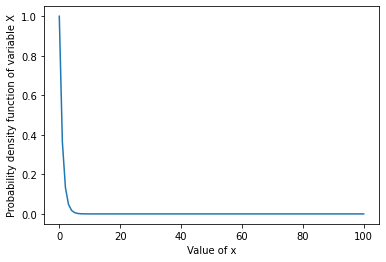
\includegraphics[width=\columnwidth]{solutions/2013/june/42/figures/figure2.png}
%     \caption{P.D.F. of X }
%     \label{june2013-42:june2013-42:fig:fig_label}
% \end{figure}
Let $f_X(x)$ denote the probability distribution function for random variable X.
\begin{align}
f_{X}(x)=
 \begin{cases} 
      \lambda_X  e^{-\lambda_X  x} & x \geq 0 \\
      0 & otherwise
 \end{cases}
\end{align}
Let $f_Y(y)$ denote the probability distribution function for random variable Y.
\begin{align}
f_{Y}(y)=
 \begin{cases} 
      \lambda_Y  e^{-\lambda_Y  y} & y \geq 0 \\
      0 & otherwise
 \end{cases}
 \end{align}
 Let $F_X(x)$ denote the cumulative distribution function for random variable X.
\begin{align}
F_{X}(x)=
 \begin{cases} 
      1-e^{-\lambda_X  x} & x \geq 0 \\
      0 & otherwise
 \end{cases}
\end{align}
Let $F_Y(y)$ denote the cumulative distribution function for random variable Y.
\begin{align}
F_{Y}(y)=
 \begin{cases} 
      1-e^{-\lambda_Y  y} & y \geq 0 \\
      0 & otherwise
 \end{cases}
 \end{align}
\begin{equation}\label{june2013-42:meanx}
    E(X)=\dfrac{1}{\lambda_X}
\end{equation}
\begin{equation}\label{june2013-42:meany}
    E(Y)=\dfrac{1}{\lambda_Y}
\end{equation}
From \ref{june2013-42:meanx} and \ref{june2013-42:meany},
\begin{equation}\label{june2013-42:lambda}
    \lambda_X = \lambda_Y = 1
\end{equation}
\begin{figure}[h]
    \centering
    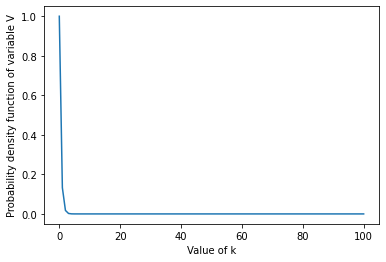
\includegraphics[width=\columnwidth]{solutions/2013/june/42/figures/figure.png}
    \caption{Parallel system}
    \label{june2013-42:fig:fig_label}
\end{figure}
Let Z be a random variable such that $Z=max(X,Y)$
\begin{align}
    P(Z\leq z) &= P(max(X,Y) \leq z)
    \\
    &=P(X\leq z,Y\leq z)
    \\
    &=P(X\leq z) P(Y\leq z)
    \\
    &=(F_X(z)-F_X(0)) (F_Y(z)-F_Y(0))
    \\
    &=1-e^{-(\lambda_X) z}-e^{-(\lambda_Y) z}+e^{-(\lambda_X+\lambda_Y) z}
\end{align}
$P(Z\leq z)$ denotes the probability that the system dies in the first $z$ seconds.\\
\begin{align}
    Expectation &= \int_{0}^{\infty}z \,d(P(Z\leq z))
    \\
\nonumber    &=\int_{0}^{\infty}z(\lambda_Xe^{-(\lambda_X) z}+\lambda_Ye^{-(\lambda_Y) z}\\
&-(\lambda_X+\lambda_Y)e^{-(\lambda_X+\lambda_Y) z}) \,dz
    \\
    &= \dfrac{1}{\lambda_X}+\dfrac{1}{\lambda_Y}-\dfrac{1}{\lambda_X+\lambda_Y}
\end{align}
From \ref{june2013-42:lambda}, 
\begin{equation}
    Expectation=\dfrac{3}{2}
\end{equation}
Therefore, option C correct.

%
\item Let $X_1$,$X_2$,... be independent random variables each following exponential distribution with mean 1. Then which of the following statements are correct?
\begin{enumerate}
    \item P($X_n > \log n$ for infinitely many $n \geq 1$) = 1
    \item P($X_n > 2$ for infinitely many $n \geq 1$) = 1
    \item P($X_n > \frac{1}{2}$ for infinitely many $n \geq 1$) = 0
    \item P($X_n > \log n, X_{n+1}>\log (n+1)$ for infinitely many $n \geq 1$) = 0
\end{enumerate}
%
\solution
\newcommand{\Integral}[2]{\ensuremath{\int\limits_{#1}^{#2}}}
PDF of $X_i$ is
\begin{align}
    f_{X_i}(x)=\begin{cases}\lambda_i e^{-\lambda_i x}, &x\geq 0\\
                0, &x<0\nonumber
    \end{cases}    
\end{align} 
Mean of $X_i$ is expressed as
\begin{align}
    \mean{X_i}&=\Integral{-\infty}{\infty}x f_{X_i}(x) dx\nonumber\\
              &=\Integral{-\infty}{0}0 dx + \Integral{0}{\infty}x \lambda_i e^{-\lambda_i x}\nonumber\\
              &=\frac{1}{\lambda_i}\label{june/2013/101a}
\end{align}
From \eqref{june/2013/101a}and $\mean{X_i}=1$, we have $\lambda_i=1 \forall  i \geq1$
Now, for some constant $c\geq0$
\begin{align}
    \pr{X_n>c}&=\Integral{c}{\infty}f_{X_n}(x)dx\nonumber\\
              &=\Integral{c}{\infty}e^{-x}dx\nonumber\\
              %&=-e^{-x}\Big|_c^{\infty}\nonumber\\
              &=e^{-c}\label{june/2013/101b}
\end{align}
\textbf{Borel-Cantelli Lemma}:\\
Let $E_1$,$E_2$,... be a sequence of events in some probability space. The Borel–Cantelli lemma states that, if the sum of the probabilities of the events $E_n$ is finite
\begin{align}
    \sum_{n=1}^{\infty}\pr{E_n}&<\infty
\end{align}
then the probability that infinitely many of them occur is 0
\begin{align}
    \pr{\lim_{n \rightarrow \infty}\sup E_n}&=0
\end{align}
\textbf{Second Borel-Cantelli Lemma}:\\
If the events $E_n$ are independent and the sum of the probabilities of the $E_n$ diverges to infinity, then the probability that infinitely many of them occur is 1.
If for independent events $E_1,E_2,...$
\begin{align}
    \sum_{n=1}^{\infty}\pr{E_n}&=\infty
\end{align}
Then
\begin{align}
    \pr{\lim_{n \rightarrow \infty}\sup E_n}&=1
\end{align}
\bigskip
\begin{enumerate}
    \item \textbf{Option 1:} 
    We can say the events $X_n>\log n$ are independent $\forall n\geq 1$ as $X_n$ are independent random variable.
    
    From \eqref{june/2013/101b}
    \begin{align}
        \sum_{n=1}^{\infty}\pr{X_n > \log n} &=\sum_{n=1}^{\infty}e^{-\log n}\nonumber\\ &=\sum_{n=1}^{\infty}\frac{1}{n}\nonumber\\
                                            &= \infty  \text{ (Cauchy's Criterion)}\nonumber
    \end{align}
    Now, from second Borel-Cantelli lemma
    \begin{align}
        &\pr{X_n>\log n \text{ for infinitely many }n\geq1}\nonumber\\
        &=\pr{\lim_{n \rightarrow \infty}\sup X_n>\log n}\nonumber\\
        &=1\nonumber
    \end{align}
    $\therefore$ Option 1 is correct. 
    
    \item\textbf{Option 2:} We can say the events $X_n>2$ are independent $\forall n\geq 1$ as $X_n$ are independent random variable.
    
    From \eqref{june/2013/101b}
    \begin{align}
        \sum_{n=1}^{\infty}\pr{X_n > 2} &= \sum_{n=1}^{\infty}e^{-2}\nonumber\\
                                            &= \infty\nonumber
    \end{align}
    Now, from second Borel-Cantelli lemma
    \begin{align}
        &\pr{X_n>2 \text{ for infinitely many }n\geq1}\nonumber\\
        &=\pr{\lim_{n \rightarrow \infty}\sup X_n>2}\nonumber\\
        &=1\nonumber
    \end{align}
    $\therefore$ Option 2 is correct.
    
    \item \textbf{Option 3:} We can say the events $X_n>\frac{1}{2}$ are independent $\forall n\geq 1$ as $X_n$ are independent random variable.
    
    From \eqref{june/2013/101b}
    \begin{align}
        \sum_{n=1}^{\infty}\pr{X_n > \frac{1}{2}} &= \sum_{n=1}^{\infty}e^{-\frac{1}{2}}\nonumber\\
                                            &= \infty\nonumber
    \end{align}
    Now, from second Borel-Cantelli lemma
    \begin{align}
        &\pr{X_n>\frac{1}{2} \text{ for infinitely many }n\geq1}\nonumber\\
        &=\pr{\lim_{n \rightarrow \infty}\sup X_n>\frac{1}{2}}\nonumber\\
        &=1\nonumber
    \end{align}
    $\therefore$ Option 3 is incorrect.
    \item \textbf{Option 4:} We can say the events $X_n>\log n$ are independent $\forall n\geq 1$ as $X_n$ are independent random variable.
    
    Let the event $X_n > \log n,X_{n+1}>\log (n+1)$ be represented by $E_n$'
    
    From \eqref{june/2013/101b}
    \begin{align}
        &\sum_{n=1}^{\infty}\pr{E_n}\nonumber\\
        &= \sum_{n=1}^{\infty}\pr{X_n>\log n}\pr{X_{n+1}>\log (n+1)}\nonumber\\
        &=\sum_{n=1}^{\infty}e^{-\log n}e^{-\log (n+1)}\nonumber\\
        &=\sum_{n=1}^{\infty}\frac{1}{n(n+1)}\nonumber\\
        &=\sum_{n=1}^{\infty}\frac{1}{n}-\frac{1}{n+1}\nonumber\\
        &=1
    \end{align}
    Now, from Borel-Cantelli lemma
    \begin{align}
        &\pr{E_n\text{ for infinitely many }n\geq1}\nonumber\\
        &=\pr{\lim_{n \rightarrow \infty}\sup ( X_n>\log n,X_{n+1}>\log (n+1))}\nonumber\\
        &=0\nonumber
    \end{align}
    $\therefore$ Option 4 is correct.
\end{enumerate}
\vspace{0.5cm}\centering \boxed{\solution{\text{Options 1, 2, 4}}}
%
\item Suppose $X_1$ and $X_2$ are independent and identically distributed random variables each following an exponential distribution with mean $\theta$, i.e., the common pdf is given by $f_\theta(x) = \frac{1}{\theta}e^{\frac{-x}{\theta}}, 0<x<\infty,0<\theta<\infty.$ Then which of the following is true? Conditional distribution of $X_2$ given $X_1+X_2=t$ is 
\begin{enumerate}
    \item exponential with mean $\frac{t}{2}$ and hence $X_1+X_2$ is sufficient for $\theta$ \label{june/2013/40/option 1}
    \item exponential with mean $\frac{t\theta}{2}$ and hence $X_1+X_2$ is not sufficient for $\theta$ \label{june/2013/40/option 2}
    \item uniform$(0,t)$ and hence $X_1+X_2$ is sufficient for $\theta$ \label{june/2013/40/option 3}
    \item uniform$(0,t\theta)$ and hence $X_1+X_2$ is not sufficient for $\theta$ \label{june/2013/40/option 4}
\end{enumerate}
%
\solution
Let $f_{X_1,X_2}(x_1,x_2)$ denote the joint probability distribution of random variables $X_1$ and $X_2$. Let $Z$ be another random variable such that $Z=X_1+X_2$. Let $\Phi_{X_1}(\omega)$ and $\Phi_{Z}(\omega)$ be the characteristic functions of the probability density functions $f_{X_1}(x)$ and $f_{Z}(x)$ respectively. The conditional probability density function of $X_2$ can be defined by:
\begin{align}
    f_{X_2|(X_1+X_2=t)}(x_2) &= 
    \begin{cases}
    \frac{f_{X_1,X_2}(x_1,x_2)}{f_{(X_1+X_2)}(t)} &  \text{if }x_1+x_2=t\\ ~\\[-1em]
    0 & \text{otherwise}
    \end{cases}
    \\ x_1 + x_2 &= t
    \\ 0 < x_1, x_2&< \infty \label{june/2013/40/equation 2}
    \\ x_1 &= t-x_2
    \\ t - x_2 &> 0
    \\ x_2 &< t \label{june/2013/40/equation 3}
\end{align}
From equations \eqref{june/2013/40/equation 2} and \eqref{june/2013/40/equation 3}, we can conclude that $x_2 \in (0, t)$ if $x_1+x_2=t$. Also, given in the question,
\begin{align}
    0 &< \theta < \infty
    \\f_{X_1}(x_1) &= \frac{1}{\theta}e^{\frac{-x_1}{\theta}}, 0<x_1<\infty
    \\f_{X_2}(x_2) &= \frac{1}{\theta}e^{\frac{-x_2}{\theta}}, 0<x_2<\infty
\end{align}
Since $X_1$ and $X_2$ are independent, 
\begin{align}
f_{X_1,X_2}(x_1,x_2) &= f_{X_1}(x_1) \times f_{X_2}(x_2)
    \\&= \frac{1}{\theta}e^{\frac{-x_1}{\theta}} \times \frac{1}{\theta}e^{\frac{-x_2}{\theta}}
    \\&= \frac{1}{\theta^2}e^{\frac{-(x_1+x_2)}{\theta}}
    \\\Phi_{X_1}(\omega) &= \frac{1}{\theta} \int_{0}^{\infty}e^{i\omega x} e^{\frac{-x}{\theta}} \,dx
    \\ &= \frac{1}{\theta} \times \frac{1}{i\omega - \frac{1}{\theta}} \brak{e^{x(i\omega - \frac{1}{\theta}}}\bigg\vert_0^{\infty}
    \\ &= \frac{1}{1-i\omega\theta} - \frac{\lim_{x\rightarrow \infty} \brak{e^{x(i\omega - \frac{1}{\theta}}}}{1-i\omega\theta}
    \\&= \frac{1}{1-i\omega\theta} - 0 = \frac{1}{1-i\omega\theta} 
    \\ \Phi_{Z}(\omega) &= \brak{\frac{1}{1-i\omega\theta} }^2
    \\ f_Z(x) &= \frac{1}{2\pi} \int_{-\infty}^{\infty}\frac{e^{-i\omega x}}{\brak{\frac{1}{1-i\omega\theta} }^2} \,d\omega \label{june/2013/40/equation 1}
\end{align}
The equation \eqref{june/2013/40/equation 1} is the characteristic function expression of a gamma random variable with k=2. Thus,
\begin{align}
    f_Z(x) &= \frac{x^{k-1}e^{\frac{-x}{\theta}}}{\Gamma(k)\theta^k}
    \\ &=  \frac{x^{2-1}e^{\frac{-x}{\theta}}}{\Gamma(2)\theta^2}
    \\ &= \frac{xe^{\frac{-x}{\theta}}}{\theta^2}
\end{align}
\begin{align}
    f_{X_2|(X_1+X_2=t)}(x_2) = 
    \begin{cases}
    \frac{f_{X_1,X_2}(x_1,x_2)}{f_Z(t)} &  x_2 \in (0, t)\\ ~\\[-1em]
    0 & \text{otherwise}
    \end{cases}
\end{align}
Let $ x_2 \in (0, t)$.
\begin{align}
    f_{X_2|(X_1+X_2=t)}(x_2) &= \frac{f_{X_1,X_2}(x_1,x_2)}{f_Z(t)}
    \\&= \frac{\frac{1}{\theta^2}e^{\frac{-(x_1+x_2)}{\theta}}}{\frac{1}{\theta^2}e^{\frac{-t}{\theta}}t}
    \\&= \frac{e^{\frac{-(t)}{\theta}}}{e^{\frac{-t}{\theta}}t}
    \\&= \frac{1}{t} \quad \forall x_2 \in (0, t)
\end{align}
The obtained pdf is uniform$(0,t)$. Any distribution is sufficient for underlying parameter $\theta$ if the conditional probability distribution of the data does not depend on the parameter $\theta$.  And since the conditional distribution of $X_2$ does not depend on $\theta$ for any value of $t$, $X_1+X_2$ is sufficient for $\theta$. Verifying the pdf,
\begin{align}
    \text{total probability} &= \int_{0}^{t} f_{X_2|(X_1+X_2=t)}(x_2) \,dx_2
    \\&= \int_{0}^{t} \frac{1}{t} \,dx_2
    \\&= 1
\end{align}
Hence, the correct answer is option \eqref{june/2013/40/option 3}
%
\item Let $X_{1},X_{2},\dots$ be independent and identically distributed random variables each following a uniform distribution on (0,1). Denote $T_{n}=max\{ X_{1},X_{2},\dots,X_{n}\}$. Then, which of the following statements are true?
\begin{enumerate}
    \item $T_{n}$ converges to 1 in probability.
    \item $n(1-T_{n})$ converges in distribution.
    \item $n^{2}(1-T_{n})$ converges in distribution.
    \item $\sqrt{n}(1-T_{n})$ converges to 0 in probability.
\end{enumerate}
%
\solution
The PDF, CDF of each $X_{1},X_{2},X_{3},\dots$ is 
\begin{align}
\tag{72.1}
    f_{X_{i}}(x)=\begin{cases}
	1, & 0< x<1 \\~\\[-1em]
	0, & otherwise
	\end{cases} 
\end{align}
\begin{align}
\tag{72.2}
	F_{X_{i}}(x)=\begin{cases}
	x, & 0< x<1 \\~\\[-1em]
	1, & x\geq 1\\~\\[-1em]
	0, & otherwise
	\end{cases} 
\end{align}
$\forall i\in \mathbb{N}$.
Then, as $T_{n}=max\{ X_{1},X_{2},\dots,X_{n}\}$,
\begin{align}
\tag{72.3}
    f_{T_{n}}(x)=\begin{cases}
	nx^{n-1}, & 0< x<1 \\~\\[-1em]
	0, & otherwise
	\end{cases} \\
\tag{72.4}
	F_{T_{n}}(x)=\begin{cases}
	x^{n}, & 0< x<1 \\~\\[-1em]
	1, & x\geq 1\\~\\[-1em]
	0, & otherwise
	\end{cases} 
\end{align}
NOTE : If $Y=aX+b$ and $a<0$, then
\begin{align}
\tag{72.5}
\label{june/2013/72/eq:form}
    F_{Y}(y)=1-F_{X}\brak{\dfrac{y-b}{a}}
\end{align}
\begin{enumerate}
\item OPTION-1:\\
Convergence in Probability :\\
A sequence of random variables $X_{1},X_{2},X_{3},\dots$ converges in probability to a random variable $X$, shown by $X_{n}\xrightarrow[]{p}X$, if
\begin{align}
\tag{72.6}
    \displaystyle\lim_{n\to\infty}\pr{|X_{n}-X|\geq\epsilon}=0,\forall\epsilon>0
\end{align}
To evaluate : $\displaystyle\lim_{n\to\infty}\pr{|T_{n}-1|\geq\epsilon},\forall\epsilon>0$
\begin{align}
\tag{72.7}
    &\displaystyle\lim_{n\to\infty}\pr{|T_{n}-1|\geq\epsilon}=\displaystyle\lim_{n\to\infty}\pr{1-T_{n}\geq\epsilon}\\
\tag{72.8}
    &=\displaystyle\lim_{n\to\infty}\pr{T_{n}\leq1-\epsilon}=\displaystyle\lim_{n\to\infty}F_{T_{n}}(1-\epsilon)
\end{align}
\begin{align}
\tag{72.9}
    F_{T_{n}}(1-\epsilon)=\begin{cases}
	(1-\epsilon)^{n}, & 0< \epsilon<1 \\~\\[-1em]
	0, & \epsilon\geq 1
	\end{cases}
\end{align}
\begin{align}
\tag{72.10}
    \because\displaystyle\lim_{n\to\infty}(1-\epsilon)^{n}=0 \text{ for } 0< \epsilon<1\\
    \tag{72.11}
    \therefore \displaystyle\lim_{n\to\infty}\pr{|T_{n}-1|\geq\epsilon}=0,\forall\epsilon>0
\end{align}
$\therefore T_{n}$ converges to 1 in probability.
\item OPTION-2:\\
Convergence in Distribution :\\
A sequence of random variables $X_{1},X_{2},X_{3},\dots$ converges in distribution to a random variable $X$, shown by $X_{n}\xrightarrow[]{d}X$, if
\begin{align}
\tag{72.12}
    \displaystyle\lim_{n\to\infty}F_{X_{n}}(x)=F_{X}(x)
\end{align}
for all $x$ at which $F_{X}(x)$ is continuous.\\
To evaluate : $\displaystyle\lim_{n\to\infty}F_{n(1-T_{n})}(x)$\\ 
Substituting $a=-n,b=n$ in \eqref{june/2013/72/eq:form},
\begin{align}
\tag{72.13}
    F_{n(1-T_{n})}(x)=1-F_{T_{n}}\brak{1-\dfrac{x}{n}}
\end{align}
\begin{align}
\tag{72.14}
    F_{T_{n}}\brak{1-\dfrac{x}{n}}=\begin{cases}
	\brak{1-\dfrac{x}{n}}^{n}, & 0< x<n \\~\\[-1em]
	1, & x\leq 0\\~\\[-1em]
	0, & x\geq n
	\end{cases} 
\end{align}
\begin{align}
\tag{72.15}
    \because\displaystyle\lim_{n\to\infty}\brak{1-\dfrac{y}{n}}^{n}=e^{-y}
\end{align}
\begin{align}
\tag{72.16}
\label{june/2013/72/eq:bcdf}
    \therefore\displaystyle\lim_{n\to\infty} F_{T_{n}}\brak{1-\dfrac{x}{n}}=\begin{cases}
	e^{-x}, & 0< x<n \\~\\[-1em]
	1, & x\leq 0\\~\\[-1em]
	0, & x\geq n
	\end{cases} 
\end{align}
\begin{align}
\tag{72.17}
\label{june/2013/72/eq:cdf}
    \therefore F_{n(1-T_{n})}(x)=\begin{cases}
	1-e^{-x}, & 0< x<n \\~\\[-1em]
	0, & x\leq 0\\~\\[-1em]
	1, & x\geq n
	\end{cases} 
\end{align}
\begin{figure}[h!]
\centering
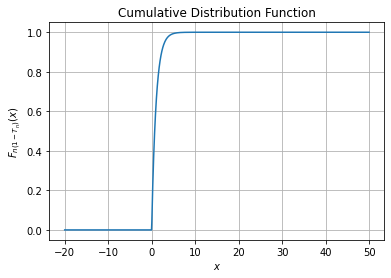
\includegraphics[width=\columnwidth]{solutions/2013/june/72/figures/Assignment9}
\caption{CDF}
\label{june/2013/72/plot}
\end{figure}
$\therefore n(1-T_{n})$ converges in distribution to a random variable with CDF in \eqref{june/2013/72/eq:cdf}.
\item OPTION-3:\\
Convergence in Distribution :\\
A sequence of random variables $X_{1},X_{2},X_{3},\dots$ converges in distribution to a random variable $X$, shown by $X_{n}\xrightarrow[]{d}X$, if
\begin{align}
\tag{72.18}
    \displaystyle\lim_{n\to\infty}F_{X_{n}}(x)=F_{X}(x)
\end{align}
for all $x$ at which $F_{X}(x)$ is continuous.\\
To evaluate : $\displaystyle\lim_{n\to\infty}F_{n^{2}(1-T_{n})}(x)$\\ 
Substituting $a=-n^{2},b=n^{2}$ in \eqref{june/2013/72/eq:form},
\begin{align}
\tag{72.19}
    F_{n^{2}(1-T_{n})}(x)=1-F_{T_{n}}\brak{1-\dfrac{x}{n^{2}}}
\end{align}
\begin{align}
\tag{72.20}
    F_{T_{n}}\brak{1-\dfrac{x}{n^{2}}}=\begin{cases}
	\brak{1-\dfrac{x}{n^{2}}}^{n}, & 0< x<n^{2} \\~\\[-1em]
	1, & x\leq 0\\~\\[-1em]
	0, & x\geq n^{2}
	\end{cases} 
\end{align}
\begin{align}
\tag{72.21}
    \because\displaystyle\lim_{n\to\infty}\brak{1-\dfrac{y}{n^{2}}}^{n}\text{ is not defined}
\end{align}
$\therefore n^{2}(1-T_{n})$ does not converge in distribution.
\item OPTION-4:\\
Convergence in Probability :\\
A sequence of random variables $X_{1},X_{2},X_{3},\dots$ converges in probability to a random variable $X$, shown by $X_{n}\xrightarrow[]{p}X$, if
\begin{align}
\tag{72.22}
    \displaystyle\lim_{n\to\infty}\pr{|X_{n}-X|\geq\epsilon}=0,\forall\epsilon>0
\end{align}
To evaluate :\\ $\displaystyle\lim_{n\to\infty}\pr{|\sqrt{n}(1-T_{n})-0|\geq\epsilon},\forall\epsilon>0$
\begin{align}
\tag{72.23}
    =\displaystyle\lim_{n\to\infty}\pr{1-T_{n}\geq\dfrac{\epsilon}{\sqrt{n}}}\\
\tag{72.24}
    =\displaystyle\lim_{n\to\infty}\pr{T_{n}\leq1-\dfrac{\epsilon}{\sqrt{n}}}\\
\tag{72.25}
    =\displaystyle\lim_{n\to\infty}F_{T_{n}}\brak{ 1-\dfrac{\epsilon}{\sqrt{n}}}
\end{align}
\begin{align}
\tag{72.26}
    F_{T_{n}}\brak{1-\dfrac{\epsilon}{\sqrt{n}}}=\begin{cases}
	\brak{1-\dfrac{\epsilon}{\sqrt{n}}}^{n}, & 0< \epsilon< \sqrt{n}\\~\\[-1em]
	0, & \epsilon\geq \sqrt{n}
	\end{cases}
\end{align}
\begin{align}
\tag{72.27}
    \because\displaystyle\lim_{n\to\infty}\brak{1-\dfrac{\epsilon}{\sqrt{n}}}^{n}=0 \text{ for } 0< \epsilon<\sqrt{n}\\
    \tag{72.28}
    \therefore \displaystyle\lim_{n\to\infty}\pr{|\sqrt{n}(1-T_{n})-0|\geq\epsilon}=0,\forall\epsilon>0
\end{align}
$\therefore\sqrt{n}(1-T_{n})$ converges to 0 in probability.
\end{enumerate}
\begin{lstlisting}
Hence, options 1), 2), 4) are correct.
\end{lstlisting}

\end{enumerate}
